\chapter{Results}
\label{chap:results}

 The data taken has been compared with 7 commonly used transport theoretical models. These models took part in a large collaborative effort in order to standardize certain common elements of each models \cite{theoryComp1,theoryComp2}. To reduce uncertainties in the pion production mechanism, each model simulated nuclear matter in a box type simulation with fixed, well defined, initial conditions. Though these box calculations model an equilibrated system at finite density, which is  not replicated by experiment, the solutions  of  pion and $\Delta$ yields can be analytically calculated from the ansatz of statistical equilibrium, providing a good benchmark. This allowed for each model to systematically go through the numerical treatment and details in each model such as initialization of nuclei, stability of the model, numerical handing of pauli-blocking, etc. After satisfying these benchmark calculations, each model was used with what each author considered the most reliable input and model assumption.  These models were taken in their best configuration, without any prior knowledge of the experimental data. We then simulated the 4 systems measured in the \spirit TPC at an impact parameter of \SI{3}{\femto\metre} at \SI{270}{\MeVA} beam energy. While the numerical treatments of each model are reasonably similar, each model differs considerably in their treatment of pion and $\Delta$ dynamics. Some models contain modifications to how the pion behaves in nuclear matter, i.e. \emph{in-medium effects}, typically introduced by including a pion optical potential, which describes the pion scattering and absorption. Some models include the iso-scalar and the iso-vector delta potential, which are not very well constrained, but can be important in the production of pions \cite{baoan_deltapotential,inmedPionKo,inmedPionFeng}. 


%It is important to note that the interaction of pions and deltas with dense matter should not be viewed as a nasty detail that a "better" probe like nucleonic elliptical flow would avoid. 
One of the central questions regarding matter at twice saturation density concerns the importance of deltas and pions as important constituents of the matter at those densities \cite{pionNS,deltaNS,awayforward}. Questions of the role of deltas and pions at 2$\rho_o$ are strongly connected to these potentials. Calculations of pion production indicate that selected pionic observables such as the energy spectra and transverse momentum distributions can be used to constrain these potentials \cite{cozmaPC}. Obtaining such constraints are a major objective of our current work, but most of these constraints have not yet been obtained.

As will be the re-occurring theme, there is a large variation in the predicted pion observables between theoretical models; this is greater than the variation between the stiff and soft symmetry energies within a particular model. However, the remedy for this discrepancy is for the authors of these models to include or better model some other physics that many of them have neglected, or it could be that the relevant physics is not constrained by other observables and needs to be constrain by further experiments and comparisons.

For example, it is clear that many models need a  better description of the delta interactions with matter, which is critical to reproducing the total pion yields, and also the momentum dependence of the isovector mean field potentials, which have a large impact on the shapes of the energy spectra. 

Other unconstrained physics includes aspects of the mean field potentials for nucleons, pions, and deltas. A primary focus is on the isovector potentials, of which only nucleon potentials for have been varied in the calculations shown below. Some of the models include the momentum dependent nucleonic mean field potentials, and the mean field potentials for deltas and pions. Calculations have already identified that the overall pion yields are influenced by the mean field potentials for the deltas \cite{cozmaPC}, which may not be surprising since a similar sensitivity has govern the occurrence of for delta and pionic matter within neutron stars \cite{deltaNS,pionNS}.  

With the \spirit TPC, we were able to measure the pion yield without resorting to extrapolations, and were able to measure the pion energy spectra of low to high energy pions accurately. In the following pages we will present the total pion yield and energy spectra for the most asymmetric systems, which complements the measurements of $\tin{112}{124}$ and $\tin{124}{112}$ collisions, which were at the focus of the dissertation of Jon Barney \cite{jon}.


\section{Pion Yield}

We begin with the total charged pion multiplicities for the two systems of extreme isospin asymmetry: the neutron rich $\tin{132}{124}$ system and the neutron deficient  $\tin{108}{112}$ system. Though the previous FOPI data set provided interesting data relevant to  the symmetry energy, they relied on extrapolations to low transverse momenta, $P_T = \sqrt{p_x^2 + p_y^2}$, below \SI{100}{\mega\electronvolt\per\clight} \cite{fopi}. In the \spirit TPC, we were able to measure pions to very low $P_T$ for rapidities $y > y{CM}$; where the rapidity is expressed along the beam direction (z) as,

\begin{equation}
y = \frac{1}{2} \ln\Big( \frac{E + p_zc}{E - p_zc}\Big).
\end{equation}

The pion rapidity in the COM system $y_{\pi CM}$ is normalized,

\begin{equation}
y_o = \frac{y_{\pi CM}}{y_{beam} - y_{CM}},
\end{equation}

where $y_{beam}$ is the beam rapidity in the lab frame and $y_{CM}$ is the CM system rapidity. This is keeping with the same notation of $y_o$ in Reference \cite{fopi}. Here $y_o = 1$ corresponds to a particle moving at beam rapidity. The   $P_T - y_o$ phase space of the \spirit TPC is plotted for both charged pions in the $\tin{132}{124}$ system , in Figure~\ref{fig:ptrap_sn132}, and the $\tin{108}{112}$ system , in Figure~\ref{fig:ptrap_sn108}. Good efficiency down to very low $P_T$ avoided any need for extrapolations. There was good acceptance of pions $y_o > 0$ -- corresponding to $\theta_{CM} < \ang{90}$ -- where we cut off the lower rapidities. This marks the first time that pions have been measured to such low $P_T$. We note that approximately 35\% of $\pi^+$ and 55\% of $\pi^-$ lie below the $P_T$ cut offs cited in the FOPI results \cite{fopi}. For the physics they were intending to do their extrapolations were sufficient, but for constraining the small effect of the symmetry energy, it is critical to measure all the way down to threshold for the pions to not introduce any extrapolation errors.

\begin{figure}[!htb]
\centering
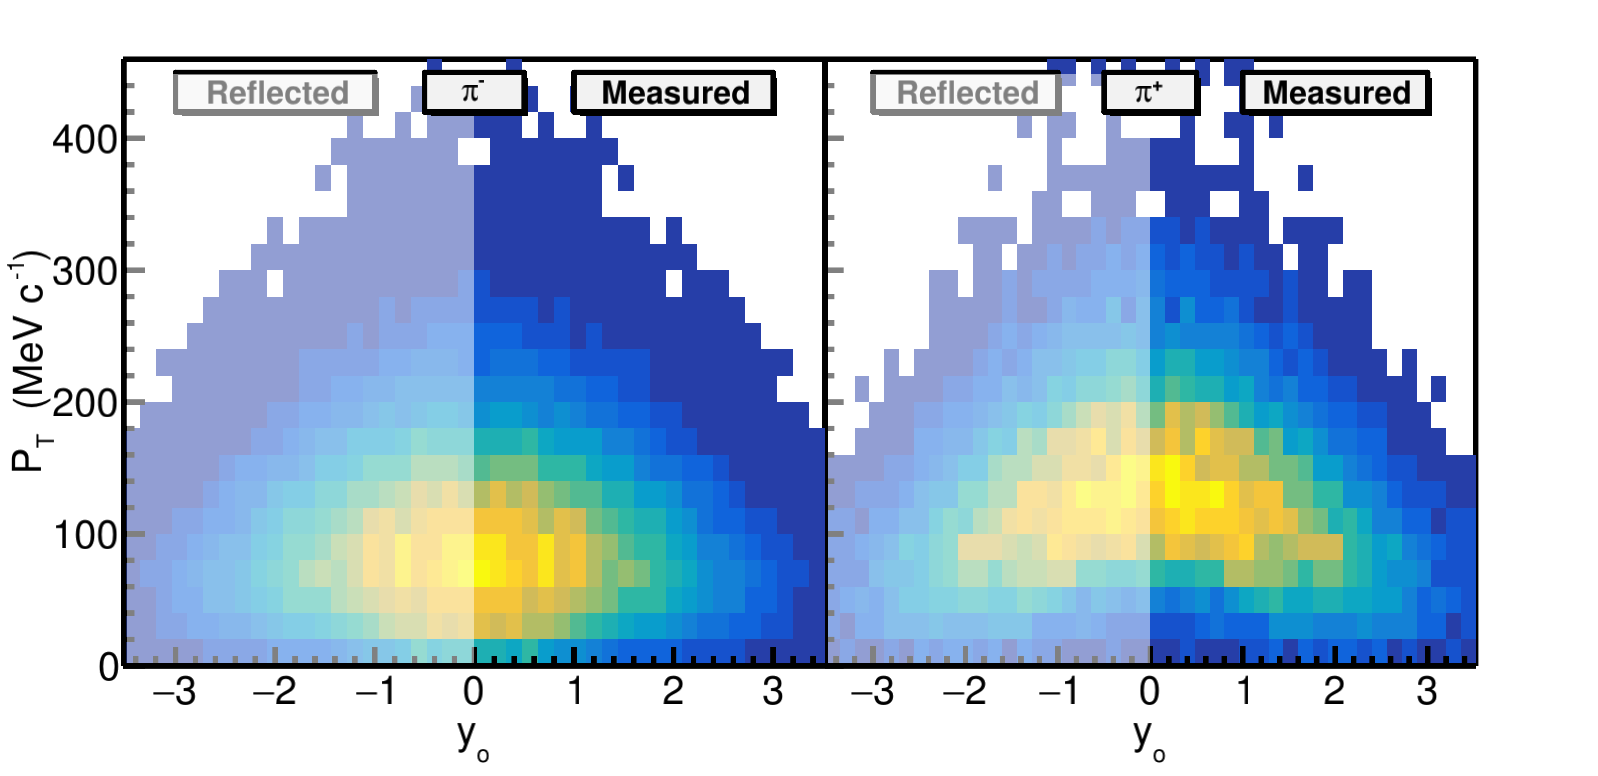
\includegraphics[width=\textwidth]{ypt_sn132.png}
\caption{Rapidity and transverse momentum plot for $\pi^-$ and $\pi^+$ in the $\tin{132}{124}$ system. The measured half of the distribution describes the forward rapidities $y_o > 0$ and has no other extrapolations. Where as the reflected side shows the measured distribution assuming symmetry about $y_o = 0$.}
\label{fig:ptrap_sn132}
\end{figure}


\begin{figure}[!htb]
\centering
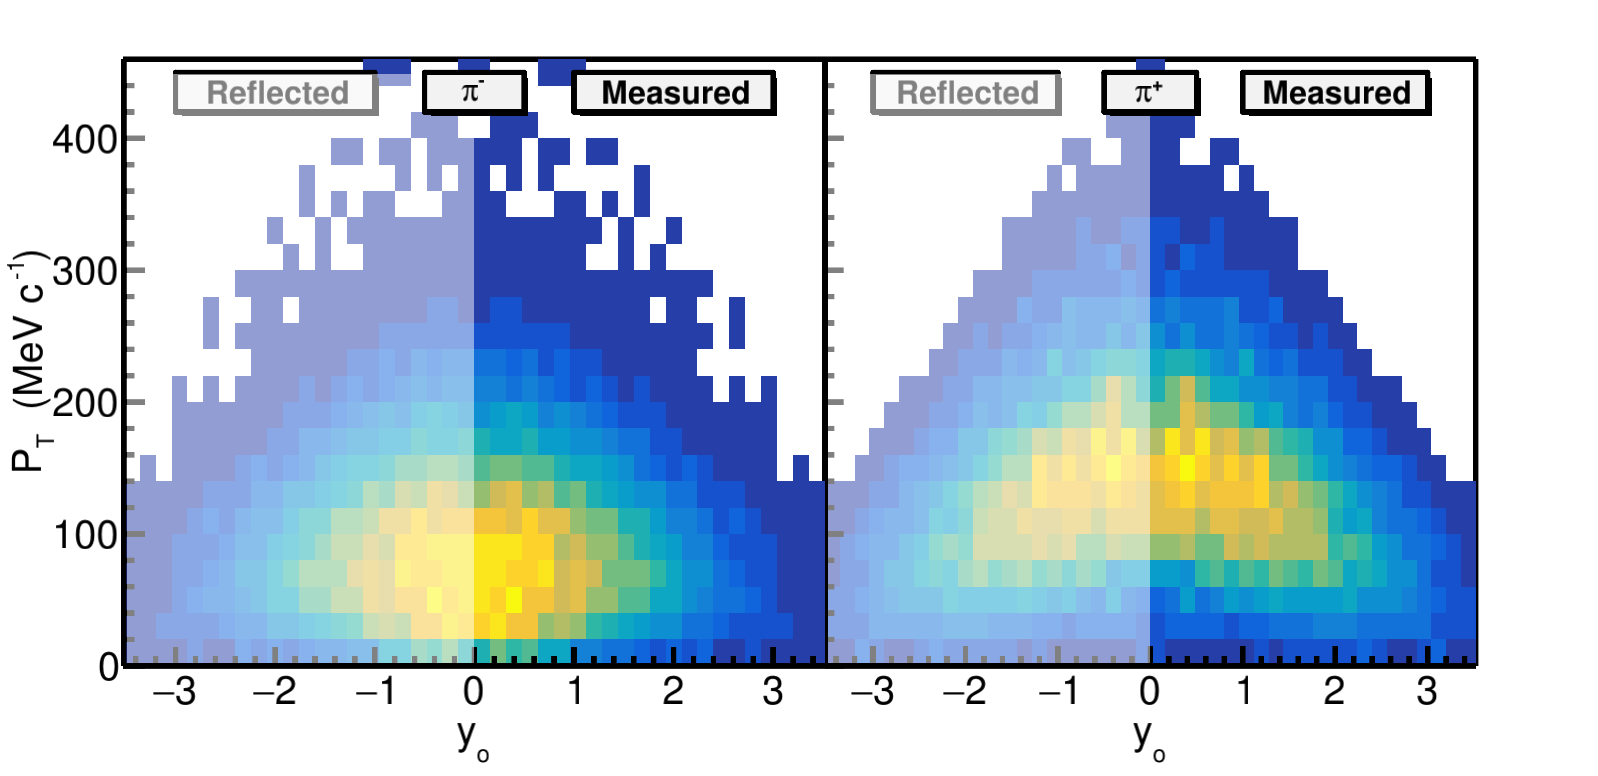
\includegraphics[width=\textwidth]{ypt_sn108.png}
\caption{Rapidity and transverse momentum plot for $\pi^-$ and $\pi^+$ in the $\tin{108}{112}$ system. The measured half of the distribution describes the forward rapidities $y_o > 0$ and has no other extrapolations. Where as the reflected side shows the measured distribution assuming symmetry about $y_o = 0$.}
\label{fig:ptrap_sn108}
\end{figure}

The integrated pion yield for both systems, and the $\pi^-/\pi^+$ ratio, is listed in Table~\ref{tb:pionyield}, where the systematic errors are the first error bar and the statistical error is listed next. This represents data with an estimated average impact parameter of $b_{avg} = \SI{2.2}{\femto\metre}$ and $b_{max} < \SI{3}{\femto\metre}$. Notice that the pion ratio is significantly greater than the $N/Z$ of the system.  This is not completely unexpected; in the delta resonance model mentioned in Section~\ref{sec:pionObs}, we expect  $\pi^-/\pi^+ \sim (N/Z)^2$ \cite{baoan_piprod1,baoan_piprod2}, where N/Z is the ratio of neutron to protons in the dense region where pions are produced. For the $\tin{132}{124}$ system $(N/Z)^2$ = 2.56 and for $\tin{108}{112}$ $(N/Z)^2$ = 1.44, but this n\"aive model assumes no migration of nucleons in or out of the high density region where the isovector mean field and other transport properties may a impact that approximation significantly. 

%Due to this connection between pion ratio and the isospin asymmetry at high density, the pion ratio was proposed to be a good probe of the isovector dynamics at high density. was hypothesized to be proportional to the high density N/Z ratio of the early system, where the other effects such as pion absorption and re-emission would dilute the effect, lowering the pion ratio as the system tends toward isospin equilibrium. It is likely however, that the dynamics plays are more significant role in pion productions via the $\Delta(1232)$ resonance than the simple $(N/Z)^2$ relation, which was also seen in \cite{fopi}. Some models assume the potential of the delta is just the same as the corresponding nucleon potential, as given by the iso-spin. While other models -- namly TuQMD -- introduce $\Delta$ resonance in-medium potential, which has an iso-scalar component (independent of iso-spin) and an iso-vector component.  These two potentials are poorly constrained, but the role they play in pion production in collisions and in neutron stars has been shown to be very important \cite{baoan_deltapotential, cozmaPC}.


\begin{table*}\centering
\ra{1.3}
\begin{tabular}{@{}cccc@{}}\toprule
System & $\pi^-$ & $\pi^+$ & $Y(\pi^-)/Y(\pi^+)$  \\
\midrule
$\tin{132}{124}$ & 0.717(24)(4) & 0.148(5)(2) & 4.84(10)(6)  \\
$\tin{108}{112}$ & 0.399(14)(3) & 0.200(8)(2) & 1.99(4)(3)  \\
%$\tin{132}{124}$ & \numerr{0.717}{0.024}{0.004} & \numerr{0.148}{0.005}{0.002} & \numerr{4.84}{0.10}{0.06}  \\
%$\tin{108}{112}$ & \numerr{0.399}{0.014}{0.003} & \numerr{0.200}{0.008}{0.002} & \numerr{1.99}{0.04}{0.03}  \\
\bottomrule
\end{tabular}
\caption{Measured total pion yield in the $\tin{132}{124}$ and $\tin{108}{112}$ systems.}
\label{tb:pionyield}
\end{table*}


We have compared the total pion yields and ratios to the 7 common transport models for the systems measured. The table of the transport models are listed in Appendix~\ref{tb:pionyieldTheory}. Figure~\ref{fig:totalpiYield} shows the total pion yield for the four systems measured as compared with the models. The models plotted here are only the soft symmetry energy since the variation in model is much larger than the variation within a model between different symmetry energies. While some models make a reasonable approximation of a particular charge pion yields, no model reasonably predicts both. 

\begin{figure}[!htb]
\centering
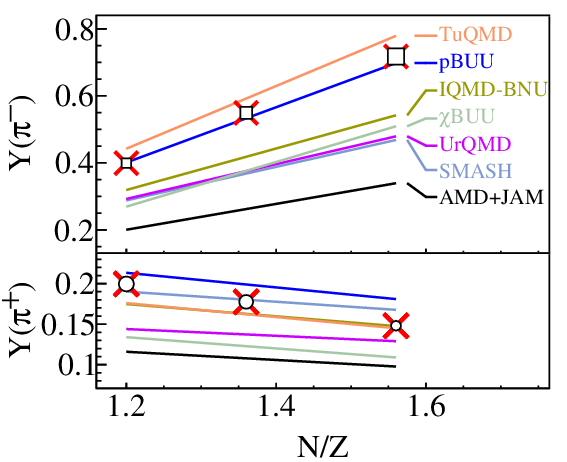
\includegraphics[width=.8\textwidth]{totalpiYield.png}
\caption{Total pion yields as compared with 7 common transport models.}
\label{fig:totalpiYield}
\end{figure}

Figure~\ref{fig:totalpiRatio} shows the total single pion ratio, $R = Y(\pi^-)/Y(\pi^+)$, and the double ratio  $DR = R_{\tin{132}{124}}/R_{\tin{124}{112}}$, of the $\tin{132}{124}$ and $\tin{108}{112}$ systems. Here, the variation between models is much larger than the variation between the momentum dependence of the symmetry energy within a particular model. The symmetry energy variation (soft and stiff extremes) of two models -- $\chi$BUU and TuQMD -- is plotted as a wide band in the single ratio and in all models in the double ratio. The circular markers and band represents the total error bar in the data. Certainly it can be seen that the variation between symmetry energy extremes in the models, though small, still exists; as initially predicted \cite{baoan_piprod1,baoan_piprod2}, and the small error bars in the data would facilitate a detailed analysis to extract the high density behavior of the symmetry energy, if not for large disagreement between models. 



\begin{figure}[!htb]
\centering
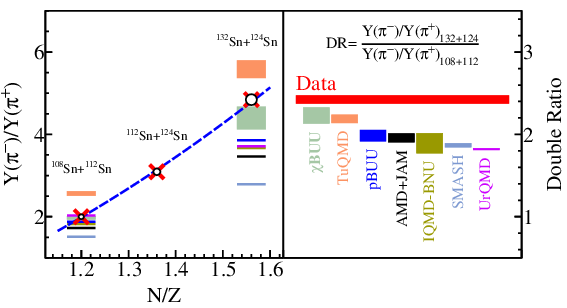
\includegraphics[width=\textwidth]{totalpiRatio.png}
\caption{Total pion ratio and double ratio compared with 7 common transport models.}
\label{fig:totalpiRatio}
\end{figure}




\section{Comparison to Previous Data Sets (FOPI)}


\begin{figure}[!htb]
\centering
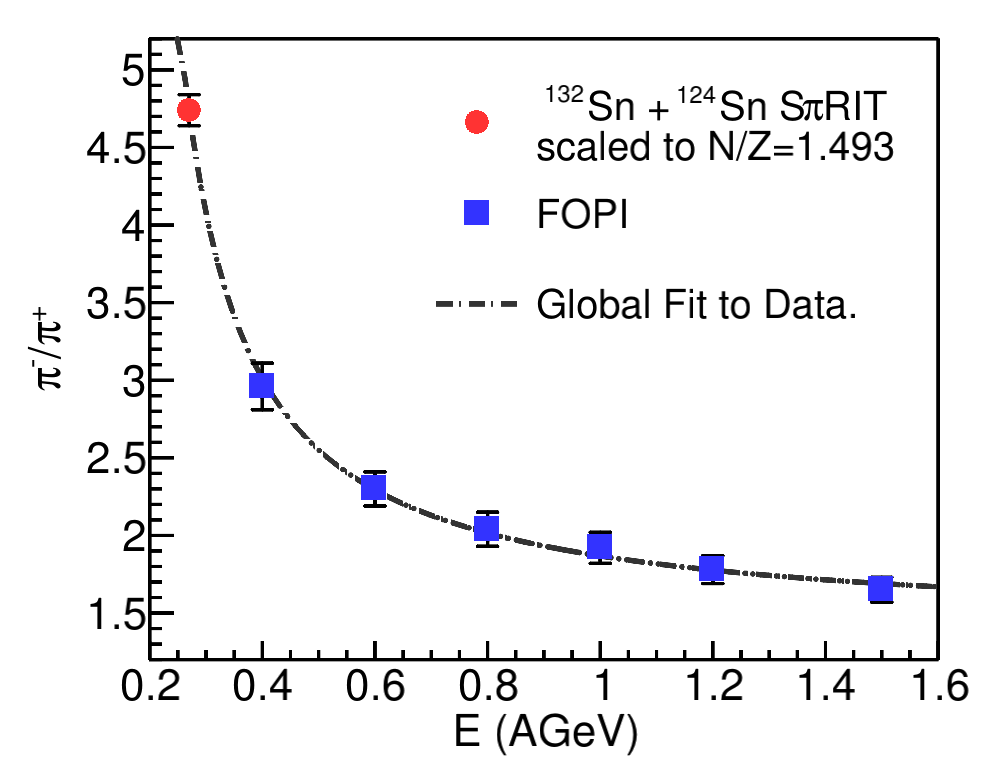
\includegraphics[scale=.4]{fopi_pionratio_comp}
\caption{Comparing the total $\pi^-/\pi^+$ ratio of the $\tin{132}{124}$ system to the ${}^{197}$Au + ${}^{197}$Au data from the FOPI collaboration. The \spirit TPC data was scaled by a factor to compare to the lower N/Z of the Au + Au system. This was extracted from measuring the N/Z dependence measured in the experiment. }
\label{fig:fopiPionRatio}
\end{figure}

The FOPI collaboration has measured the total pion multiplicity resulting from ${}^{197}Au + {}^{197}Au$ collisions at several, higher, beam energies. In the $\tin{132}{124}$ data the asymmetry is $N/Z=1.56$ where as in the ${}^{197}Au + {}^{197}Au$ the $N/Z=1.493$. Since 4 beams were measured in this experiment, the $N/Z$ dependence was measured as seen in Figure~\ref{fig:totalpiRatio}. Here the dependence is fitted with a 2-nd order polynomial fit. To compare the pion ratio in the $\tin{132}{124}$ data with that of the lower N/Z in the FOPI experiment, we scaled by the pion ratio between $N/Z=1.56$ and 1.493 as given from the fitted polynomial line. Figure~\ref{fig:fopiPionRatio} shows the scaled pion ratio as compared with the FOPI pion ratio \cite{fopi}. The fitted function has the functional form of $p_1(E - p_2)^{-2}$ where $p_1$ and $p_2$ are free parameters, and only is meant to guide the eye. It is also worth mentioning that the pion ratio observed in the FOPI \SI{400}{\MeVA} setting was already considerably higher than what is expected from the $(N/Z)^2$ delta resonance model \cite{baoan_piprod1,baoan_piprod2}. It it worth mentioning that the two experiments differ considerably in their efficiencies as was mentioned before. The FOPI results heavily relied on extrapolations to lower pion energies which the \spirit TPC did not rely on \cite{fopi}. Without a systematic error calculation or discussion with the FOPI collaboration no further detail can be given except that the \spirit TPC data seems to be reasonable expectation and in general agreement with the FOPI data set. Scaling the other systems in the \spirit TPC data leads to almost the exact same scaled value of $\mathrm{Y}(\pi^-)/\mathrm{Y}(\pi^+) = \num{4.82}$ and would be redundant. 




\section{Pion Spectra}
\label{sec:pionSpectra}


\begin{figure}[!htb]
\centering
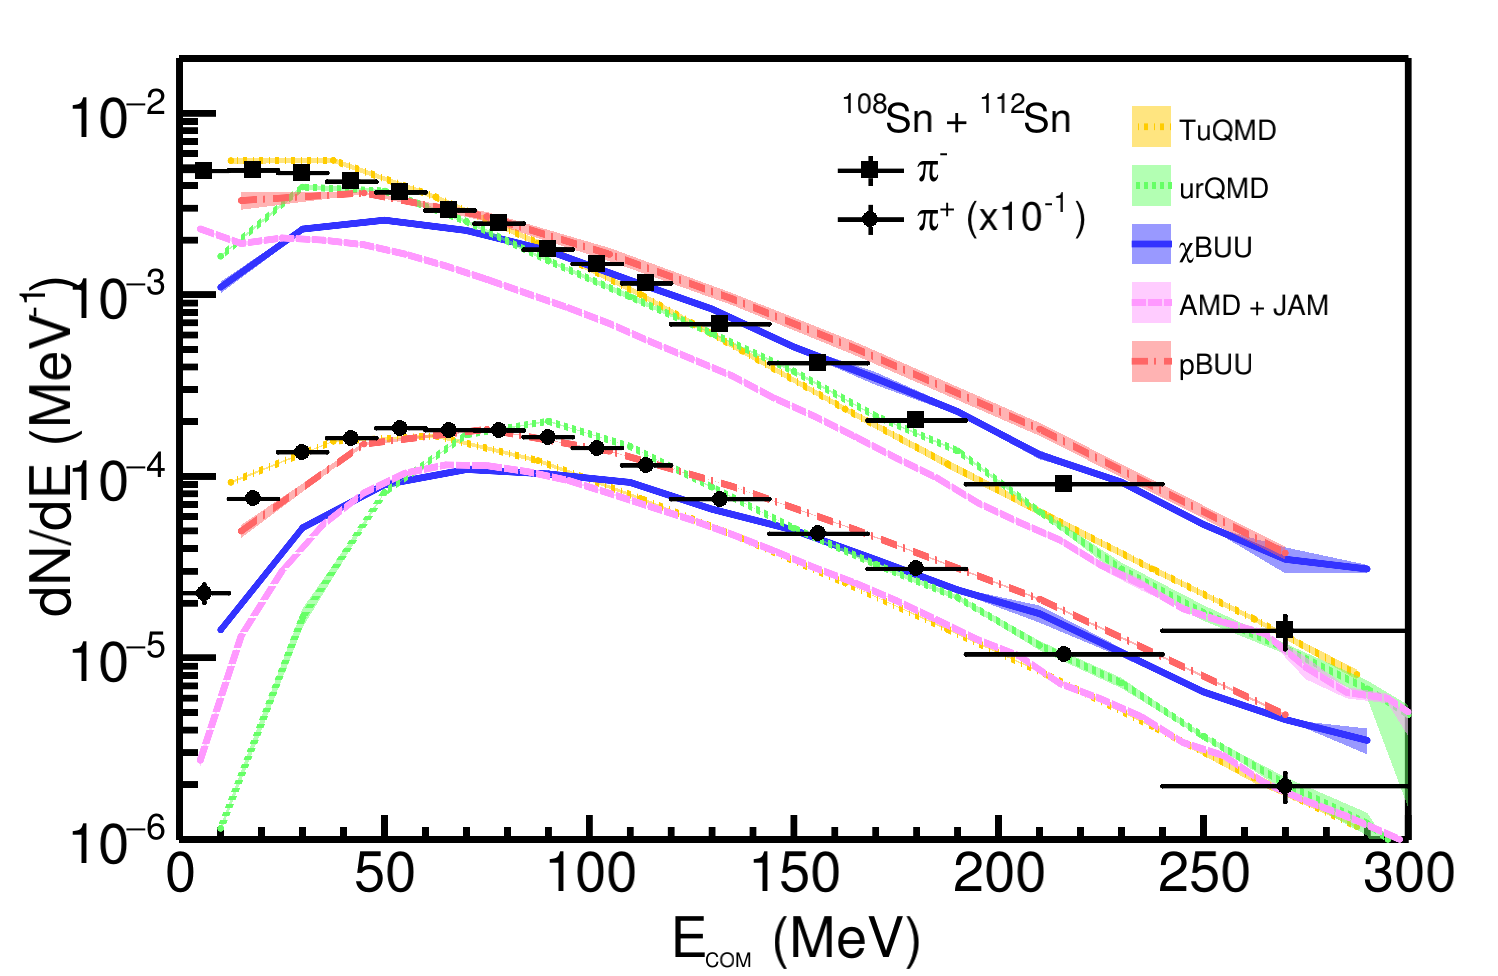
\includegraphics[width=\textwidth]{pionSpectra_sn108_sum.png}
\caption{Pion spectra for the $\tin{108}{112}$ system and comparisons to 7 theoretical models. }
\label{fig:pionspectraSn108}
\end{figure}


\begin{figure}[!htb]
\centering
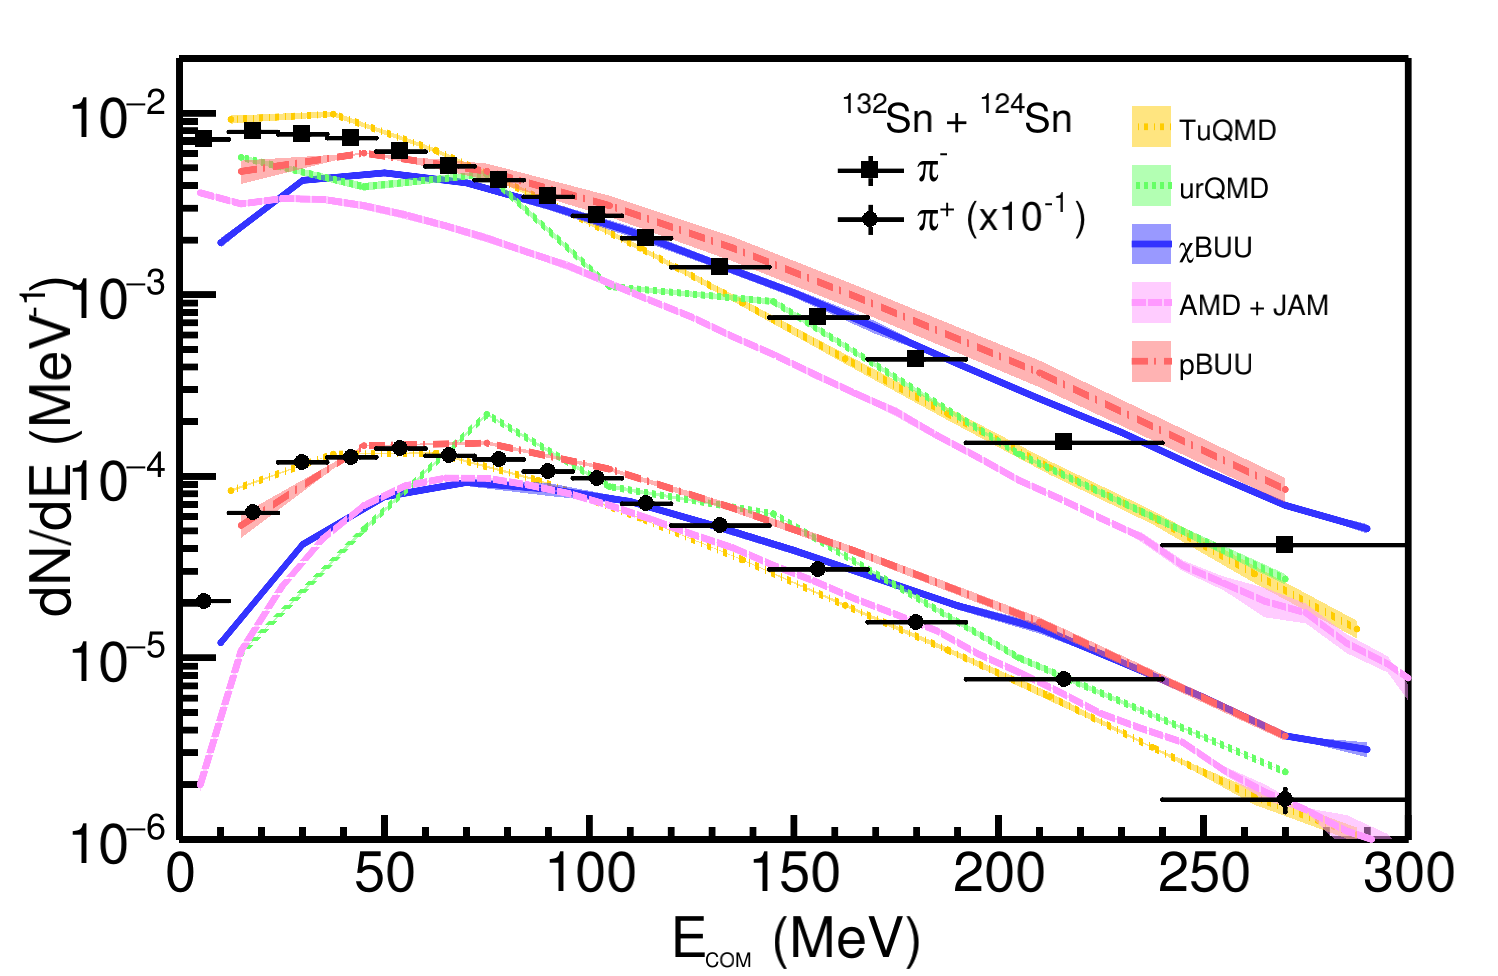
\includegraphics[width=\textwidth]{pionSpectra_sn132_sum.png}
\caption{Pion spectra for the $\tin{132}{124}$ system and comparisons to 7 theoretical models. }
\label{fig:pionspectraSn132}
\end{figure}


Figures~\ref{fig:pionspectraSn132} and \ref{fig:pionspectraSn108} shows pion CM kinetic energy spectra for both the $\tin{132}{124}$ and $\tin{108}{112}$ systems respectively; corrected for efficiency and accounting for the solid angle of 4$\pi$. This data marks the first time pion spectral data has been measured at sub-threshold energies. In the pion spectra, we can see the effect of the Coulomb potential, which accelerates $\pi^+$ and decelerates $\pi^-$ particles, due to the positive charge of the nuclear medium. The low yield for the $\pi^+$ production at low energies is caused by the Coulomb barrier between protons which limits $\pi^+$ production at low energies. The Coulomb force has the largest effect on the spectra of the pions and will play an important role when observing the general shape of the pion spectral ratio, where it changes its shape completely. 



\section{Pion Spectral Ratio}

\begin{figure}[!htb]
\centering
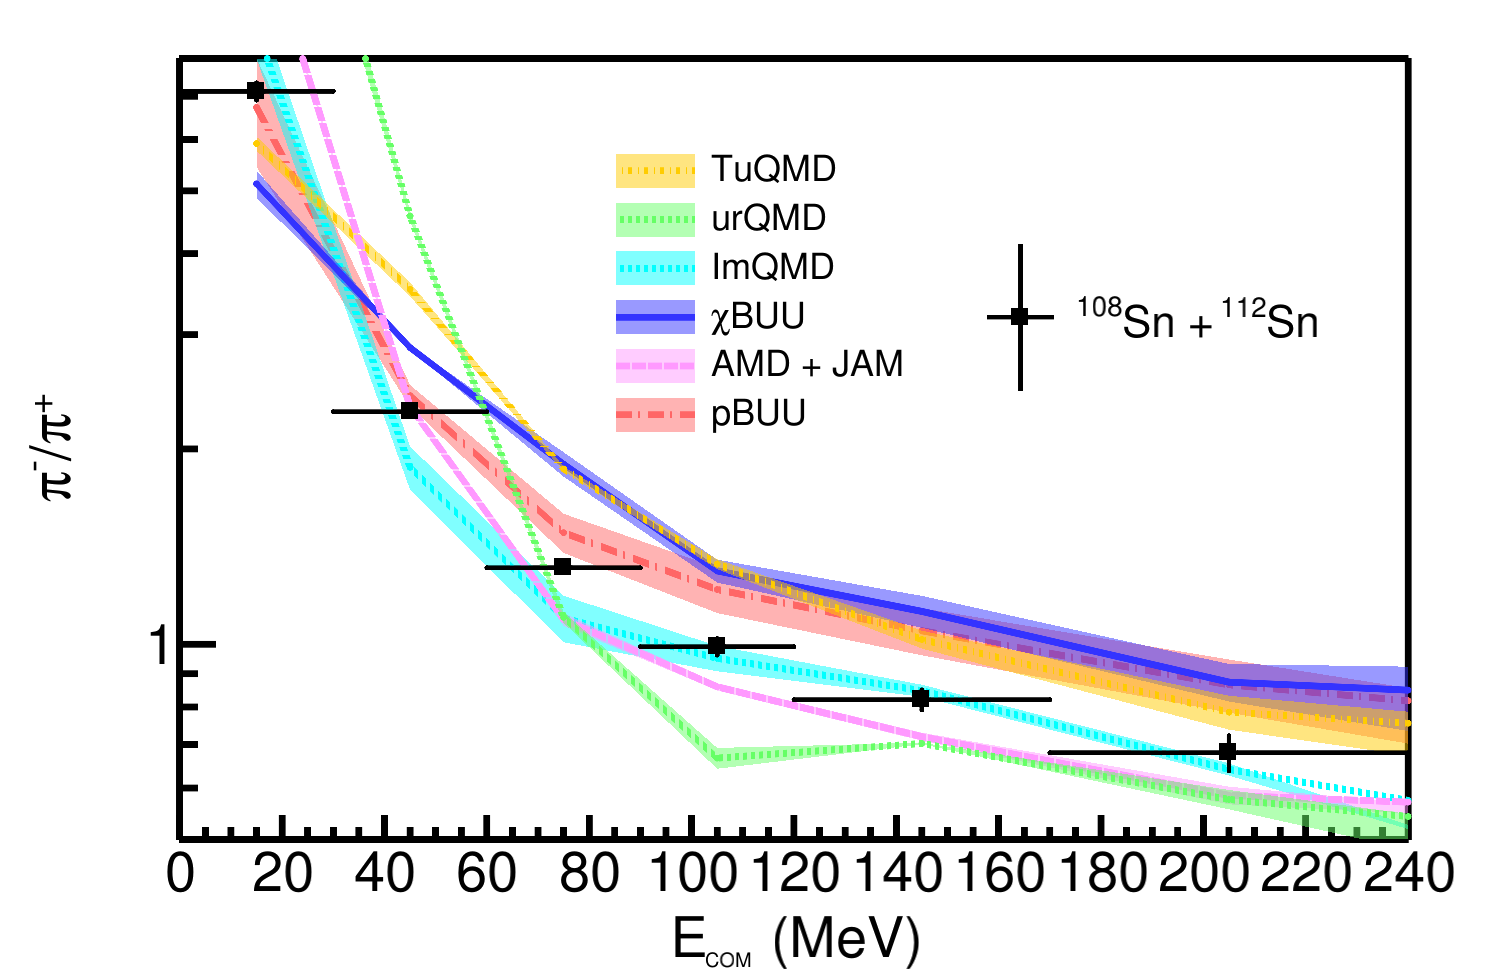
\includegraphics[width=\textwidth]{singleRatio108_log.png}
\caption{Pion spectral ratio $\tin{108}{112}$ system and comparisons to 7 theoretical models.}
\label{fig:SRsn108}
\end{figure}

\begin{figure}[!htb]
\centering
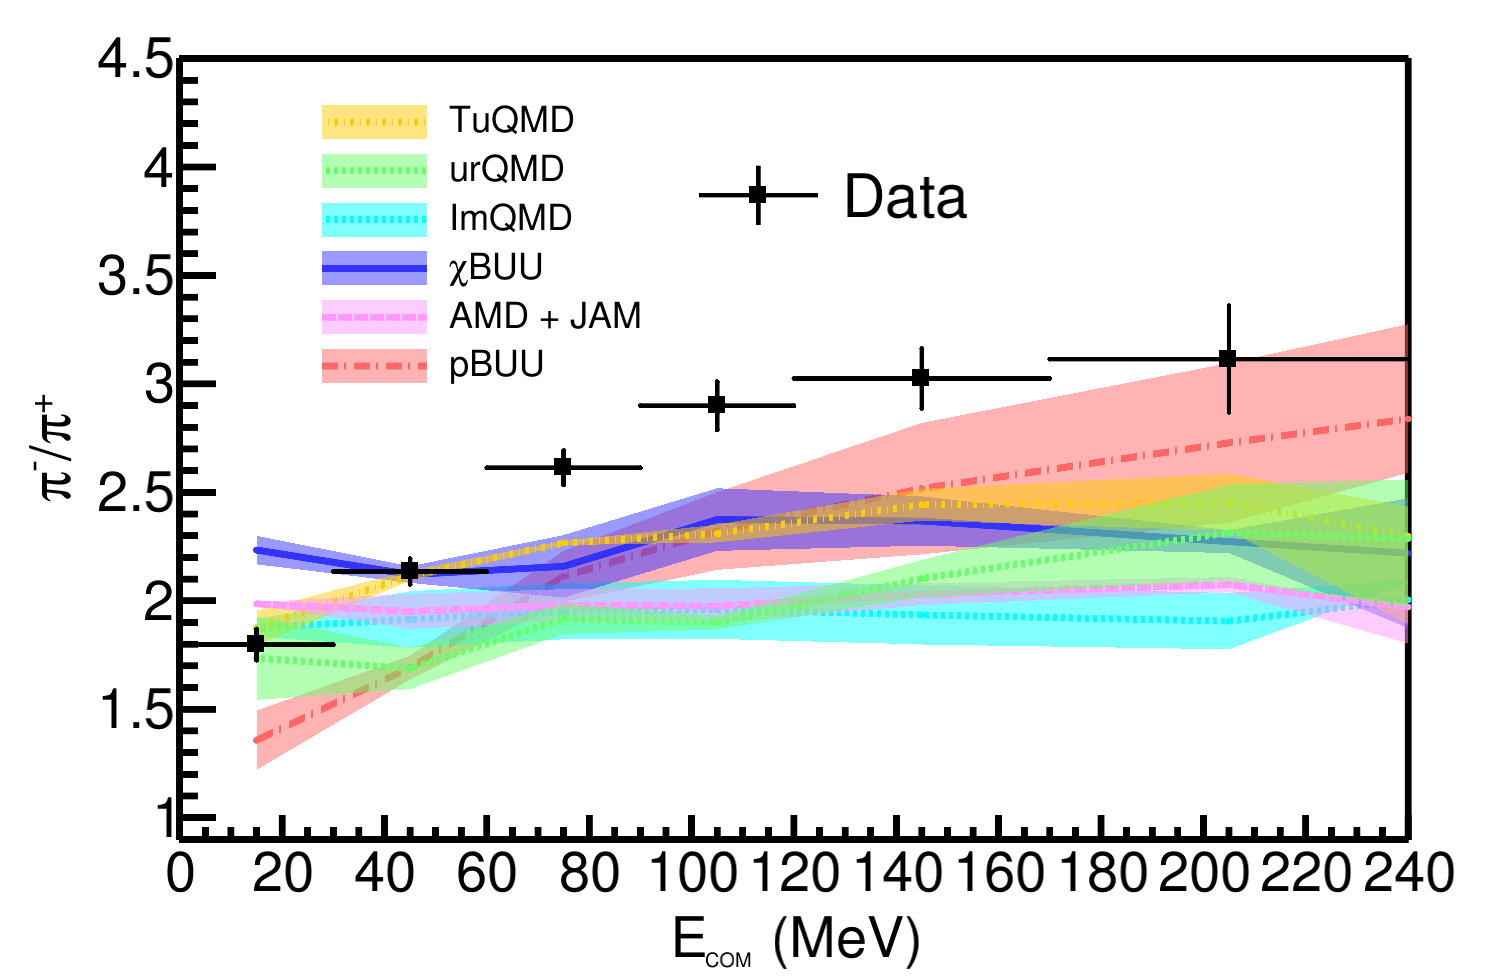
\includegraphics[width=\textwidth]{singleRatio132_sum.png}
\caption{Pion spectral ratio $\tin{132}{124}$ system and comparisons to 7 theoretical models.}
\label{fig:SRsn132}
\end{figure}

The pion spectral ratio is a rather promising observable. In particular, it may be more sensitive to the high density regions of the early collision. It is generally true that high energy pions are more likely to exit the nuclear medium  earlier, and therefore be less prone to effects such as pion absorption and re-emission; all of which dilute the sensitivity of the pion observable to the high density behavior. Conversely, low energy pions are more likely to stay in the nuclear medium, and be affected by other effects such as the $\Delta$ potential in medium \cite{baoan_deltapotential}. Integrating these two regions to get the total pion yield dilutes the possible sensitivity the high energy pions have. Instead, we can construct the $Y(\pi^-)/Y(\pi^+)$ ratio as a function of the kinetic energy in the CM system with a particular focus on high energy pions.

%Mention and cite appendix for systematics

Figure~\ref{fig:SRsn132} and \ref{fig:SRsn108} shows the pion spectral ratio for the $\tin{132}{124}$ and $\tin{108}{112}$ system respectively, which was measured with a high degree of efficiency and accuracy. The general hyperbolic shape seen in both figures arises from the Coulomb force on the two charged pion spectra mentioned earlier in Section~\ref{sec:pionSpectra}. Also notice the pion ratio is smaller for the neutron poor system, as we would expect since there are fewer neutron-neutron inelastic collisions and consequently fewer $\pi^-$. 



%Add figure of Theory for pion ratios

\section{Pion Double Ratio}
\label{sec:doubleRatio}
%Add figure of Theory for pion ratios

\begin{figure}[!htb]
\centering
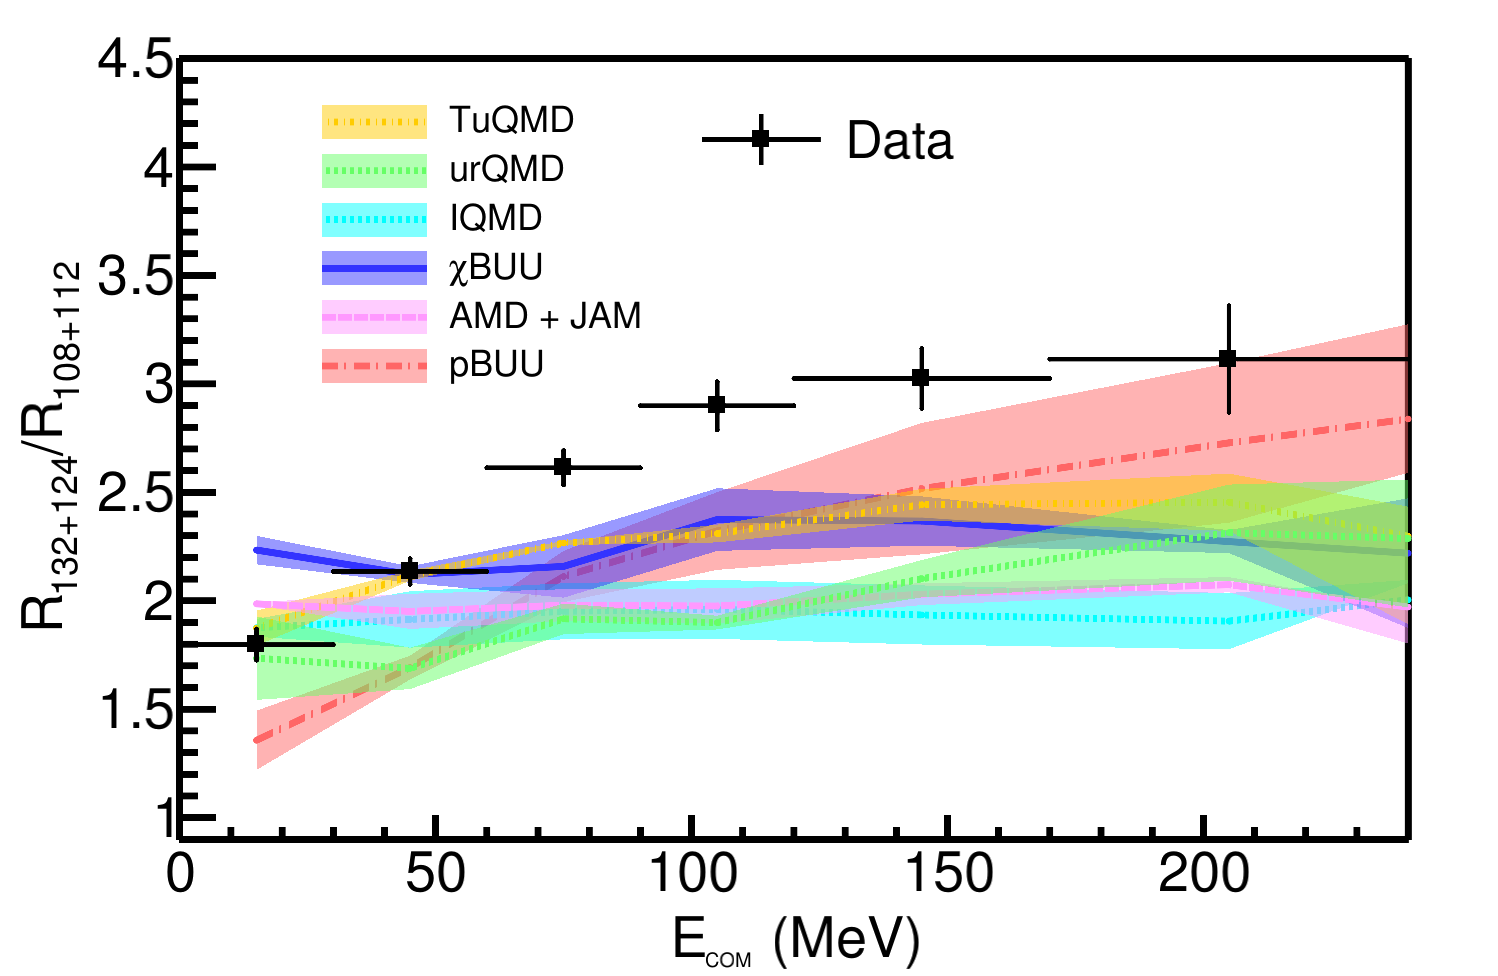
\includegraphics[width=\textwidth]{doubleRatio_sum.png}
\caption{Comparing the double spectral ratio, $R_{\tin{132}{124}}/R_{\tin{108}{112}}$, to the 7 theoretical transport simulations.}
\label{fig:spectraDR}
\end{figure}

In a similar way to the total pion double ratio, we can construct the spectral double ratio, the ratio between the two system's single ratios. As described in Section~\ref{sec:doubleRatio} we would expect systematic uncertainties in the experiment, and even in the theory --between the two systems-- to cancel out. For the same reasons as the pion spectral ratio, we would expect the high energy pions to be more sensitive to the high density region of the early collision. Here, just as in the total double ratio, the spectral double ratio is significantly higher than any theory. Here as before, the bands in the theory represent the two extremes of the symmetry energy. 
